\subsection{Hypothesis on Relation Properties}
\label{sec:hypothesis_relation_properties}

\begin{figure*}[htb]
\centering
\begin{minipage}{0.95\textwidth}
\centering
\small
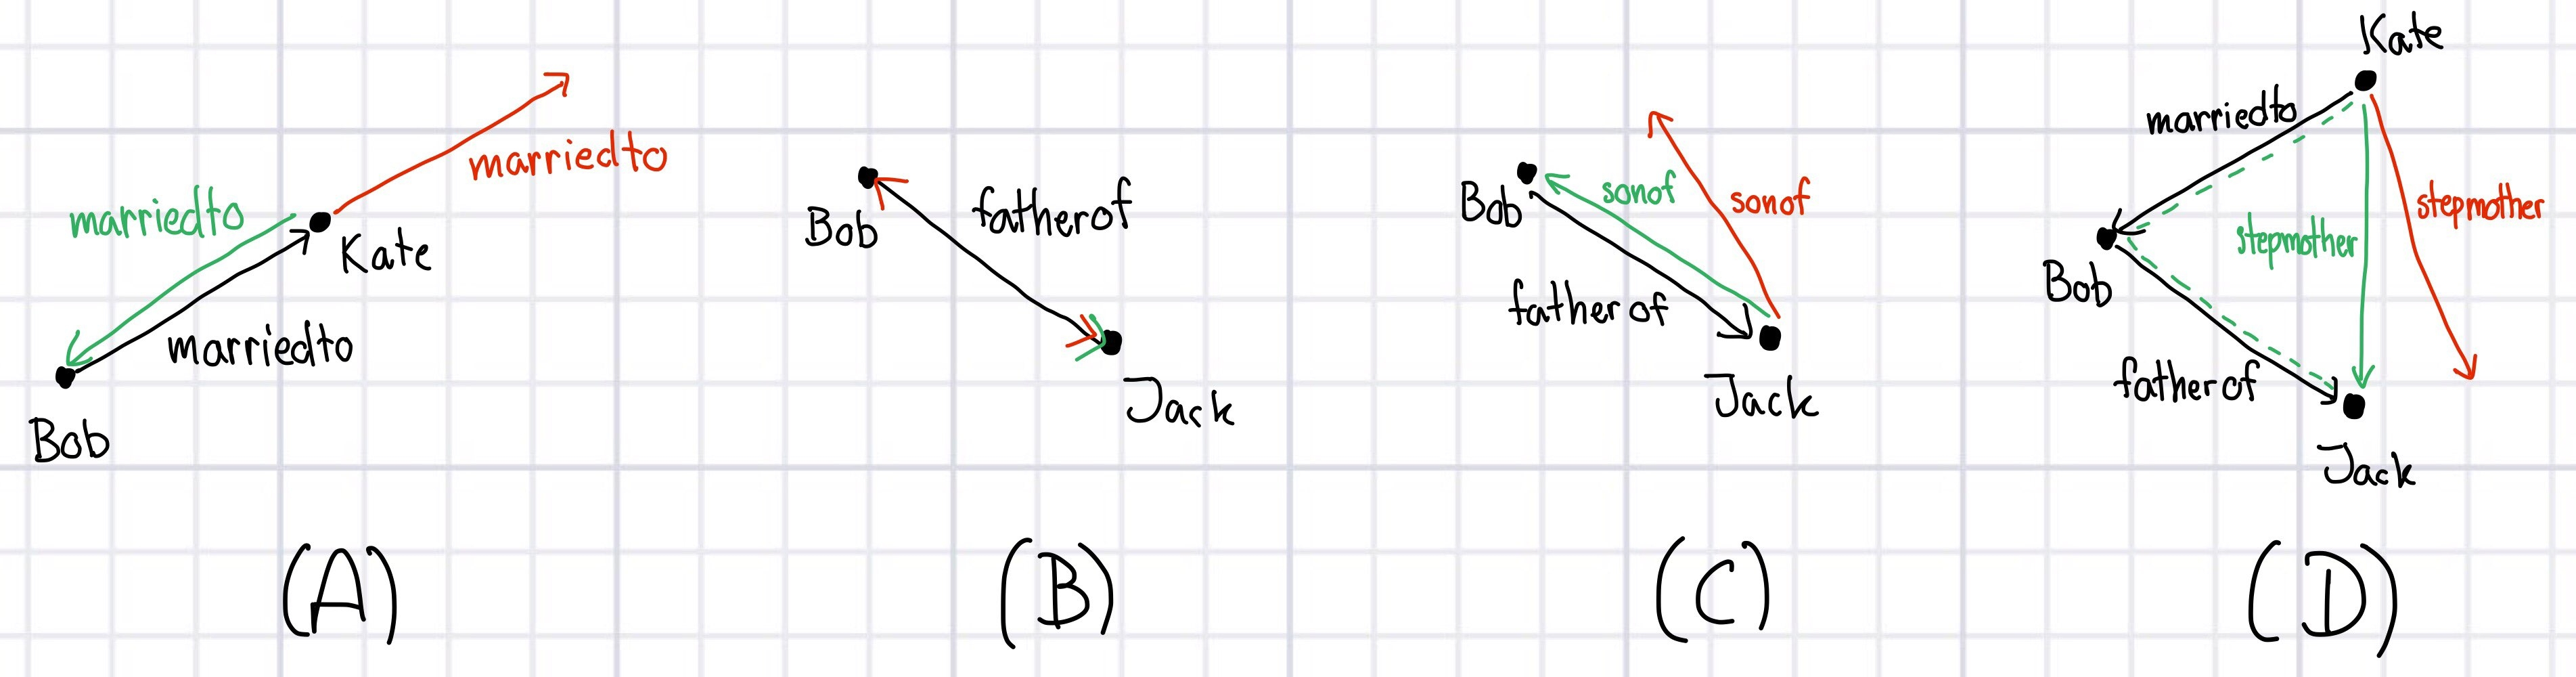
\includegraphics[scale=0.12]{content/hypotheses/figures/relation_properties_A-D.jpg}
\caption{Illustration of \autoref{hyp:relation_properties} A-D. Black is embedded information and red/green are different versions of the same relation embedding. Green is what the embedding should look like if the method can model relations with that property and red is what the embedding might look like if not. A: Symmetry, B: Anti-Symmtery, C: Inversion, D: Composition.
}
\label{fig:relation_properties_nothierarchy}
\end{minipage}
\end{figure*}

\begin{hypothesis}
\label{hyp:relation_properties}
%Prediction quality varies between models over different types of relations that are involved in the prediction task.
%Prediction quality of queries where the relation has specific properties varies between models of different embedding methods.
%Prediction quality is higher on relations with certain temporally constrained properties on methods that can express those properties, than on methods that cannot express those properties in their embeddings.
Prediction quality of queries with certain temporally constrained relation properties is better on methods, which can model those properties, than methods, which cannot.
\end{hypothesis}

This hypothesis is inspired by the fact that multiple embedding methods have been criticized for not handling or created in order to handle specific properties.
\missing[Examples]
This hypothesis is divided into several subhypotheses specific to different relation properties:

\begin{subhypothesis}
%Prediction quality of queries where the relation has the symmetry or anti-symmetry properties varies between models of different embedding methods with joint and separate entity embeddings.
Prediction quality of queries where the relation type is symmetric is higher on methods that can express symmetry than on models that can not express symmetry.
\end{subhypothesis}

This hypothesis is illustrated in \autoref{fig:relation_properties_nothierarchy} A. When Bob is married to Kate, Kate is also married to Bob. If the method cannot model symmetry it may attempt to model Kate's relation to Bob with the same vector it models Bob's relation to Kate. However, in a vector space that would point Kate's relation vector in the opposite direction.

\begin{subhypothesis}
Prediction quality of queries where the relation type is anti-symmetric is higher on methods that can express anti-symmetry than on models that can not express anti-symmetry.
\end{subhypothesis}

This hypothesis is illustrated in \autoref{fig:relation_properties_nothierarchy} B. When Bob is the father of Jack, Jack cannot be the father of Bob. If the method cannot model symmetry it may not know the direction of the vector and as such it does not know who is the father of who.

\begin{subhypothesis}
Prediction quality of queries where the relation type is the inverse of another relation type is higher on methods that can express inversion than on models that can not express inversion.
\end{subhypothesis}

This hypothesis is illustrated in \autoref{fig:relation_properties_nothierarchy} C. When Bob is the father of Jack, Jack is the son of Bob. If the method cannot model inversion it may embed the sonof relation separately from the fatherof relation and potentially get an entirely different result.

\begin{subhypothesis}
Prediction quality of queries where the relation type is a composition of a number of another relation types is higher on methods that can express composition than on models that can not express composition.
\end{subhypothesis}

This hypothesis is illustrated in \autoref{fig:relation_properties_nothierarchy} D. When Kate is married to Bob and Bob is the father of Jack, then Kate is the stepmom of Jack. Like the case for inversion, if the method cannot model composition it may embed the stepmom relation independently of its composite relations and potentially get an entirely different result.

% \begin{figure}[htb]
\centering
\begin{minipage}{0.95\columnwidth}
\centering
\small
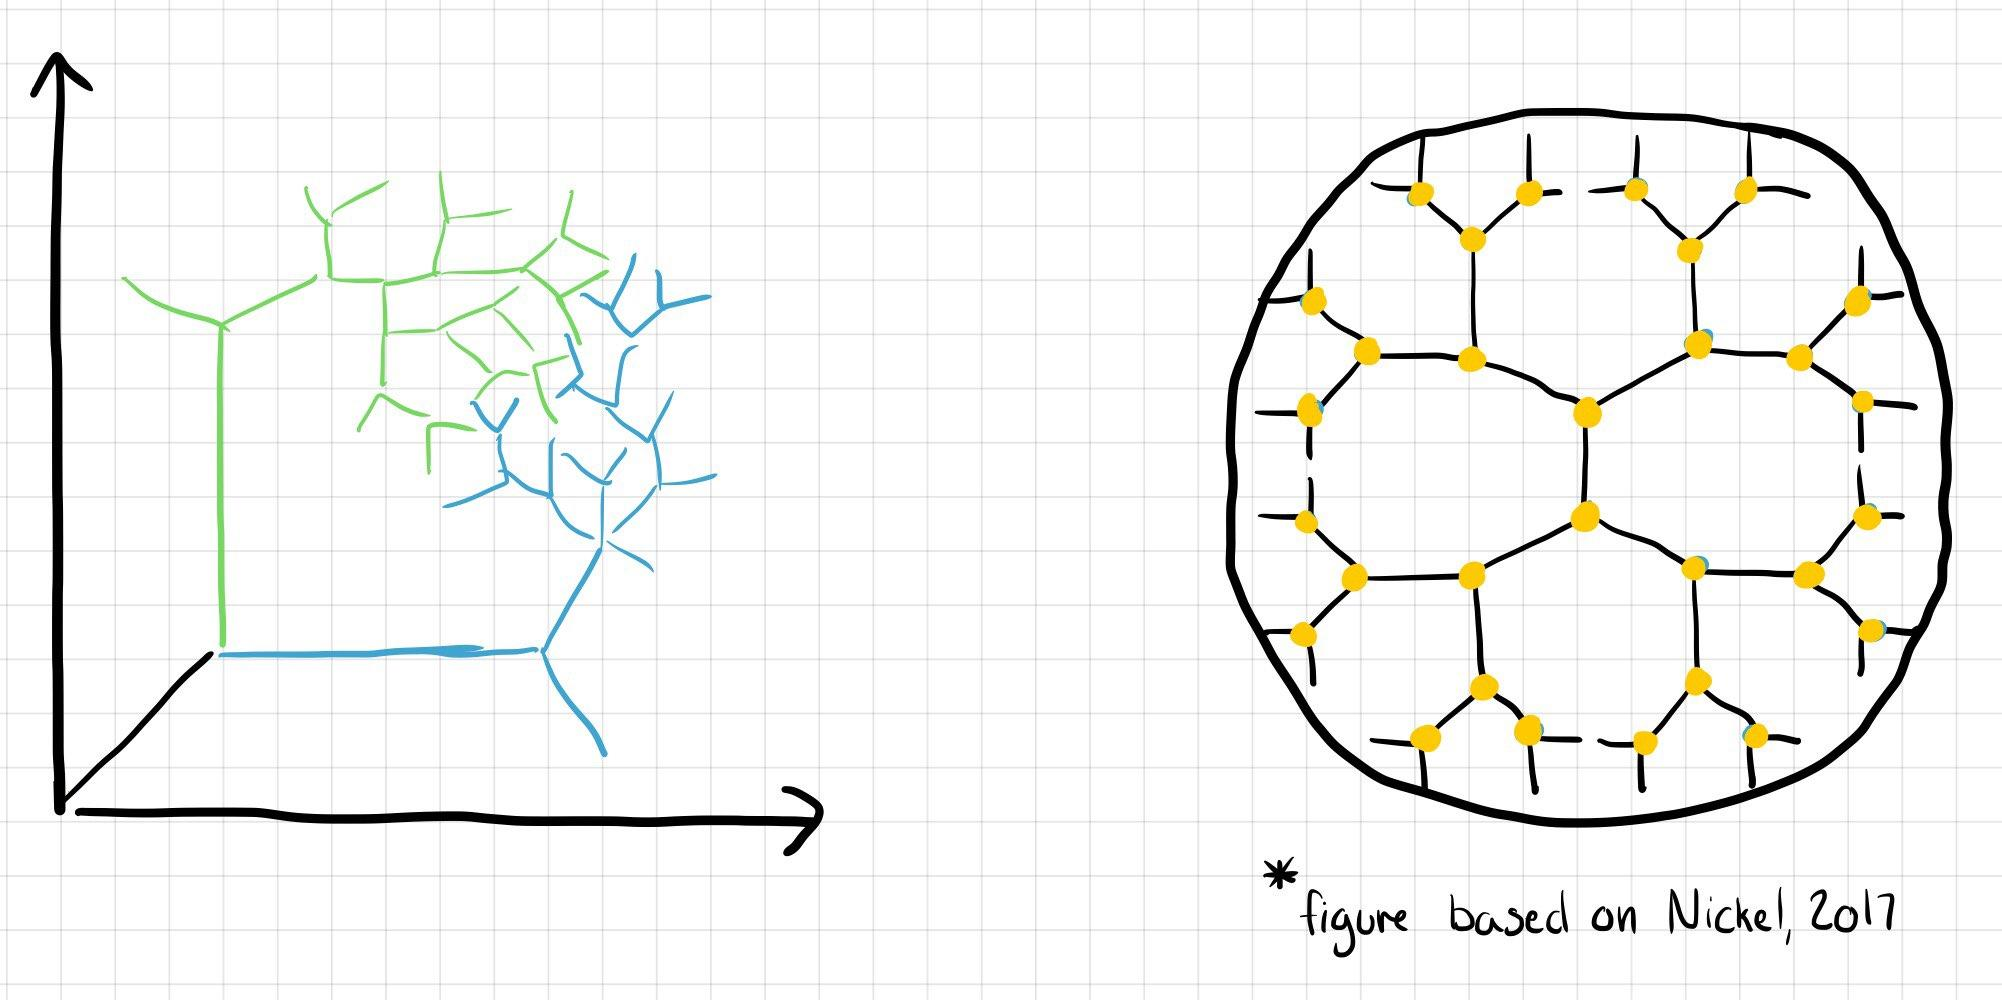
\includegraphics[scale=0.12]{content/hypotheses/figures/relation_properties_E.jpg}
\caption{Illustration of \autoref{subhyp:relation_hierarchy}. Left side shows a hierarchy embedded in Euclidian space. Right side shows a hierarchy embedded in hyperbolic space, where each yellow dot is equal distance from one another.
}
\label{fig:relation_properties_hierarchy}
\end{minipage}
\end{figure}

% \begin{subhypothesis}
% \label{subhyp:relation_hierarchy}
% Prediction quality of queries where the relation has the hierarchy property is better for models of embeddings methods within hyperbolic space.
% \end{subhypothesis}

To incorporate this in the ensemble learning method, each relation gets classified with a soft label for each relation type, using a function for each relation property that maps each relation type to a real number $\varR \rightarrow [ 0 , 1 ]$. This function describes how many relations fulfill the requirements for that relation type. The reasoning for this is that knowledge graphs are not complete, and some relations might be missing from the graph.

The soft label for symmetry for relation $r$ is

\begin{equation}
\begin{gathered}
\mathit{sym}(r) = \frac{|S|}{|\eta_r|}\\
S = \{ (e_1, r, e_2, \tau) \mid (e_1, r, e_2, \tau) \in \eta_r \wedge (e_2, r, e_1, \tau) \in \eta_r \}
\end{gathered}
\end{equation}

\noindent
The soft label for anti-symmetry for relation $r$ is

\begin{equation}
\begin{gathered}
\mathit{asym}(r) = \frac{|A|}{|\eta_r|}\\
A = \{ (e_1, r, e_2, \tau) \mid (e_1, r, e_2, \tau) \in \eta_r \wedge (e_2, r, e_1, \tau) \notin \eta_r \}
\end{gathered}
\end{equation}

\noindent
The soft label for inversion for relation $r$ is

\begin{equation}
\begin{gathered}
\mathit{inv}(r) = \varmax_{r^i \in \varR \setminus \{r\} } \frac{|I_{r^i}|}{|\eta_r|}\\
I_{r^i} = \{ (e_2, r^i, e_1, \tau) \mid (e_1, r, e_2, \tau) \in \eta_r \wedge (e_2, r^i, e_1, \tau) \in \eta_{r^i} \}
\end{gathered}
\end{equation}

\noindent
The soft label for reflexitivity for relation $r$ is

\begin{equation}
\begin{gathered}
\mathit{ref}(r) = \frac{|R|}{|\eta_r|}\\
R = \{ (e, r, e, \tau) \mid (e, r, e, \tau) \in \eta_r \}
\end{gathered}
\end{equation}

The average score for each model is then calculated for all relations that align to each of these labels, and used to calculate the most probable ranking of predictions over those relation types. The average rank of symmetrical relations on model $m$ is

%\begin{equation}
%\mathit{avg\_sym}(m) = \frac{ \varsum_{r \in \varR} \left( |\eta_r| * \mathit{sym}(r) * \frac{\varsum_{q \in \eta_r} \mathit{rank}(q , m)}{|\eta_r|} \right) }{ \varsum_{r \in \varR} |\eta_r| * \mathit{sym}(r) }
%\end{equation}

\begin{equation}
\mathit{avg\_sym}(m) = 
\frac{ \varsum_{r \in \varR} \left( \mathit{sym}(r) * \varsum_{q \in \eta_r} \frac{1}{\mathit{rank}(q , m)} \right) }
{ \varsum_{r \in \varR} |\eta_r| * \mathit{sym}(r) }
\end{equation}

\noindent
Similarly, $\mathit{avg\_asym}(m)$, $\mathit{avg\_inv}(m)$ and $\mathit{avg\_ref}(m)$ is defined, replacing $\mathit{sym}(r)$ with $\mathit{asym}(r)$, $\mathit{inv}(r)$ and $\mathit{ref}(r)$ respectively.

When a query $(h, r, t, \tau)$ is passed to the ensemble model, a weight vector $v_r \in \R^{|M|}$ is calculated for each model $m_i \in M$ from the relation $r$. This vector is defined with

\begin{equation}
v_r = \varconcat_{i = 1}^{|M|} \, \left(
\begin{aligned}
&\mathit{sym}(r) * \mathit{avg\_sym}(m_i) \, + \\
&\mathit{asym}(r) * \mathit{avg\_asym}(m_i) \, + \\
&\mathit{inv}(r) * \mathit{avg\_inv}(m_i) \, + \\
&\mathit{ref}(r) * \mathit{avg\_re}f(m_i)
\end{aligned} \right)
\end{equation}

\noindent
where $\doublepipe$ denotes concatenation between numbers, to create a vector.



